Computerspiele nutzen Multithreading seit dem Aufkommen von Mehrkern-Prozessoren, um eine bessere Perforance zu erreichen~\cite{Davies2006}. Es gibt verschiedene für Spiele geeignete Multithreading-Architekturen, die jeweils eigene Vor- und Nachteile mit sich bringen. Im folgendenden werden zwei weit verbreitete Multithreading Architekturen betrachtet.

\subsection{Thread pro System}
\todo{Entscheiden, ob auch hier gleich System on a Thread genannt}

\begin{figure}
	\centering
	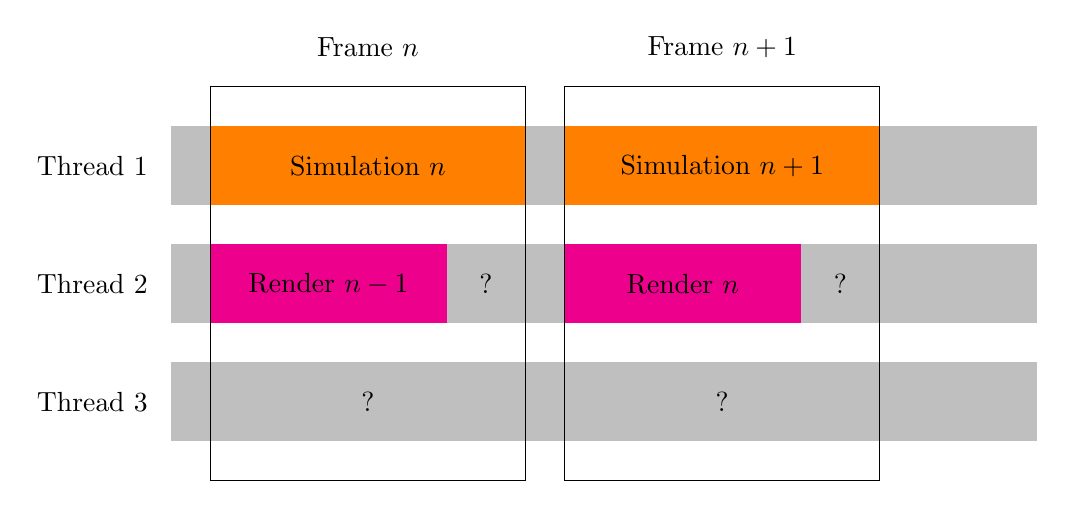
\begin{tikzpicture}
			\fill[lightgray]  (0,0) rectangle (11,1);
			\fill[lightgray] (0,-1.5) rectangle (11,-0.5);
			\fill[lightgray]  (0,1.5) rectangle (11,2.5);
			
			\node at (-1,2) {Thread 1};
			\node at (-1,0.5) {Thread 2};
			\node at (-1,-1) {Thread 3};
			
			
			\fill [orange] (0.5,2.5) rectangle (4.5,1.5);
			\fill [orange] (5,2.5) rectangle (9,1.5);
			\fill [magenta] (0.5,1) rectangle (3.5,0);
			\fill [magenta] (5,1) rectangle (8,0);
			
			
			\node at (2.5,2) {Simulation $n$};
			\node at (7,2) {Simulation $n+1$};
			\node at (2.5,3.5) {Frame $n$};
			\node at (7,3.5) {Frame $n+1$};
			
			\draw  (0.5,3) rectangle (4.5,-2);
			\draw  (5,3) rectangle (9,-2);
			
			\node at (2,0.5) {Render $n-1$};
			\node at (6.5,0.5) {Render $n$};
			\node at (4,0.5) {?};
			\node at (8.5,0.5) {?};
			\node at (2.5,-1) {?};
			\node at (7,-1) {?};
	\end{tikzpicture}
	\caption{Systeme laufen auf eigenen Threads. Es wird die Auslastung während zwei Frames $n$ und $n+$ gezeigt. Einige Threads sind dadurch nicht zu \SI{100}{\percent} ausgelastet, was durch Fragezeichen (?) gekennzeichnet ist. In diesem Fall kann Thread 3 gar nicht genutzt werden. Thread 2 übernimmt das Rendering, durch Pipelining wird dabei immer der Zustand der Simulation des letzten Frames dargestellt. Die Abbildung ist von einer Grafik aus \cite[S.~14]{Tatarchuk2014} inspiriert.}\label{fig:sot}
\end{figure}
Eine einfache Architektur vergibt, wie in Abbildung~\ref{fig:sot} gezeigt, für einzelne Systeme (wie Simulation oder Rendering) eigene Threads, die diese exklusiv nutzen~\cite{Davies2006,Tatarchuk2014,Genova2015,Hodgman2016}. \textcite{Tatarchuk2014} bezeichnet diese Architektur als \ac{sot}. Durch Pipelining kann das Rendering System dann beispielsweise auf den Spielzustand des vorherigen Frames für die Darstellung zugreifen. Diese Architektur bietet einige Vor- und Nachteile, die nun erörtert werden.
\begin{itemize}
	\item[$+$] Die Architektur bietet den Vorteil, dass die Ausführung innerhalb der Systeme seriell ist, was die Entwicklung wie in Abschnitt~\ref{sec:nebenl-folgen} beschrieben einfacher macht, als nebenläufige Entwicklung.
	\item[$+$] Solange die Systeme voneinander separiert sind, gibt es keine Probleme die mit Nebenläufigkeit einhergehen, da beispielsweise Wettkampfbedingungen nur auftreten können, wenn nebenläufig auf geteilte Daten zugegriffen wird. Da keine Wettkampfbedingungen verhindert werden müssen, entfällt (großteils) und Deadlocks sind ausgeschlossen.
	\item[$-$] Auf heterogenen Plattformen, die beispielsweise unterschiedliche Prozessoreinheiten besitzen, kann es zu Performance Problemen kommen. Die Architektur muss eventuell für jede Plattform anders aufgebaut sein. Es gibt also eine gewisse Abhängigkeit von der Hardware.
	\item[$-$] Synchronisierung der Systeme erfordert einen großen Speicheraufwand, da alle Daten (beispielsweise mit einem Double Buffer) zwischengespeichert werden müssen.
\end{itemize}

Die Nutzung von Threads pro System bietet sich an, wenn nur für eine Plattform, beispielsweise PC, entwickelt wird und es keine starken Speicherplatzrestriktionen gibt. Zudem ist die Implementierung einfacher als die der folgenden Architektur.

\subsection{Jobsystem}

\begin{figure}
	\centering
	\begin{tikzpicture}
		\fill[lightgray]  (0,0) rectangle (11,1);
		\fill[lightgray] (0,-1.5) rectangle (11,-0.5);
		\fill[lightgray]  (0,1.5) rectangle (11,2.5);
		
		\node at (-1,2) {Thread 1};
		\node at (-1,0.5) {Thread 2};
		\node at (-1,-1) {Thread 3};
	
		\foreach \i in {0,3.5,7}{
		\fill [orange,draw=lightgray] ($(\i,0) + (0.5, 1.5)$) rectangle ($(\i,0) +(1.5, 2.5)$);
		\fill [orange,draw=lightgray] ($(\i,0) + (0.5,-1.5)$) rectangle ($(\i,0) +(1.5,-0.5)$);
		\fill [orange,draw=lightgray] ($(\i,0) + (1.5, 1.5)$) rectangle ($(\i,0) +(2.5, 2.5)$);
		\fill [orange,draw=lightgray] ($(\i,0) + (0.5, 0.0)$) rectangle ($(\i,0) +(1.5, 1.0)$);
		
		\fill [magenta,draw=lightgray] ($(\i,0) + (2.5, 1.5)$) rectangle ($(\i,0) + (3.5, 2.5)$);
		\fill [magenta,draw=lightgray] ($(\i,0) + (2.5, 0.0)$) rectangle ($(\i,0) + (3.5, 1.0)$);
		\fill [magenta,draw=lightgray] ($(\i,0) + (2.5,-1.5)$) rectangle ($(\i,0) + (3.5,-0.5)$);
		
		\draw  ($(\i,0) + (0.5,3)$) rectangle ($(\i,0) + (3.5,-2)$);
		
		\node[font=\footnotesize] at ($(\i,0) + (1,2)$) {Sim 1};
		\node[font=\footnotesize] at ($(\i,0) + (1,0.5)$) {Sim 2};
		\node[font=\footnotesize] at ($(\i,0) + (1,-1)$) {Sim 3};
		\node[font=\footnotesize] at ($(\i,0) + (2,2)$) {Sim 4};
		\node[font=\footnotesize] at ($(\i,0) + (3,2)$) {Ren 1};
		\node[font=\footnotesize] at ($(\i,0) + (3,0.5)$) {Ren 2};
		\node[font=\footnotesize] at ($(\i,0) + (3,-1)$) {Ren 3};
	
		}
	\node at (2,3.5) {Frame $n$};
	\node at (5.5,3.5) {Frame $n+1$};
	\node at (9,3.5) {Frame $n+2$};
	\end{tikzpicture}
	\caption{Die Systeme definieren Jobs, die frei auf die vorhandenen Threads aufgeteilt werden. Sim steht für Simulation und Ren für Rendering. Die Abbildung ist schematisch, die Jobs müssen nicht exakt die gleiche Länge haben, auch wenn kurze Jobs mit ähnlichen Laufzeiten ideal sind. Im Vergleich zu Abbildung~\ref{fig:sot} lässt sich eine höhere Auslastung der Threads erkennen, was wiederum höhere FPS zur Folge hat.}\label{fig:jobt}
\end{figure}
\todo{Abbildung Caption}
Eine etwas komplexere Architektur liefert die Implementierung eines sogenannten \emph{Job-} oder \emph{Task-Systems}~\cite{Davies2006,Tatarchuk2014,Genova2015,Hodgman2016}. Ein Schema der Architektur ist in Abbildung~\ref{fig:jobt} zu sehen. Anstatt Aufgaben fest auf einzelne Threads zu verteilen, gibt es \emph{Jobs} und ein System, das die Jobs auf Threads verteilt. Konzeptuell entspricht die Architektur sehr dem in Abschnitt~\ref{sec:executor} beschriebenen \class{Executor} in Java. 

Die idealerweise kurzen Jobs werden an das System übergeben. Das System verwaltet die Threads, deren Anzahl idealerweise der Anzahl der Hardwarethreads entspricht, da dann die Leistung des Prozessors optimal ausgenutzt werden kann und die Anzahl der Kontextwechsel minimiert wird. Ist ein Thread im Leerlauf, wird ein Job an den Thread zur Ausführung übergeben.

\begin{figure}
	\centering
	\begin{tikzpicture}
		\node[fill=orange] (sim1) {Sim 1};
		\node[fill=orange,below=of sim1] (sim2)  {Sim 2};
		\node[fill=orange,below=of sim2] (sim3)  {Sim 3};

		\node[fill=orange,right=of sim2] (sim4)  {Sim 4};

		\node[fill=magenta,right=of sim4] (ren2)  {Ren 2};
		\node[fill=magenta,above=of ren2] (ren1)  {Ren 1};
		\node[fill=magenta,below=of ren2] (ren3)  {Ren 3};

		
		\draw[->](sim1.east) -- (sim4.north west);
		\draw[->](sim2.east) -- (sim4.west);
		\draw[->](sim3.east) -- (sim4.south west);
		\draw[->](sim4.north east) -- (ren1.west);
		\draw[->](sim4.east) -- (ren2.west);
		\draw[->](sim4.south east) -- (ren3.west);
	\end{tikzpicture}
	\caption{Beispiel eines Job Graphen, der der Ausführung in Abbildung~\ref{fig:jobt} zugrundeliegen könnte. Die farbigen Knoten stellen Jobs dar, wobei orange Knoten Simulationsjobs und magentafarbene Knoten Renderingjobs sind. Die gerichteten Kanten zeigen die mögliche Ausführungsreihen folge an. So muss beispielsweise Sim 4 nach Sim 3 ausgeführt werden. Gibt es keinen Pfad von Job $A$ zu Job $B$ so können beide parallel ausgeführt werden.}\label{fig:jobdependencies}
\end{figure}
\todo{Abbildung}
Das System kann zudem so implementiert werden, dass es Abhängigkeiten zwischen einzelnen Jobs gibt, das heißt, dass ein Job beispielsweise erst ausgeführt wird, wenn ein anderer Job abgeschlossen ist. Daraus bildet sich ein Job Graph, der die nebenläufige Ausführung der Jobs beschreibt. Es hat sich als hilfreich erwiesen, feste Synchronisationspunkte zu definieren, damit auf systemübergreifende Daten zugegriffen werden kann. Das kann im Jobsystem wie in Abbildung~\ref{fig:jobdependencies} durch Jobs repräsentiert werden, die Abhängigkeiten zu vielen vorangehenden Jobs sammeln und dann als Abhängigkeit für die folgenden Jobs dienen. Betrachten wir nun einige Vor- und Nachteile eines Jobsystems.
\begin{itemize}
	\item[$+$]  Da die Durchführung von Jobs nicht an bestimmte Threads gekoppelt ist, kann Hardware mit mehr Prozessoreinheiten sofort voll ausgenutzt werden. Wenn die Anzahl der Prozessoren zur Laufzeit ermittelt wird, funktioniert das sogar dynamisch. Ist eine Prozessoreinheite vorhanden, wird diese genutzt, gibt es $100$ Prozessorkerne, werden $100$ genutzt. Durch ein Jobsystem kann also jede beliebige in Hardware vorhandene Parallelität ausgenutzt werden. Dadurch werden ohne zusätzlichen Programmieraufwand verschiedenste Plattformen unterstützt.
	\item[$+$] Ein Jobsystem bietet die Möglichkeit, Simulation und Rendering in einem Frame sequentiell durchzuführen, ohne alle Nebenläufigkeit zu verlieren. Durch das Jobsystem können die Systeme intern parallelisiert werden. Werden Simulation und Rendering sequentialisiert, ist es nicht nötig des Spielzustand zwischenzuspeichern, da die Simulation während des Renderings bereits abgeschlossen ist und somit Wettkampfbedingungen ausgeschlossen sind (da das Rendering nur lesend auf Daten zugreift). Damit benötigt man weniger Speicher als bei einer Architektur, die auf einen Zwischenspeicher angewiesen ist. Spiele, die eh schon viel Speicher verbrauchen und auf speicherbeschränkten Systemen ausgeführt werden sollen, können auf diese Art von Nebenläufigkeit guten Gebrauch machen. 
	
	Wie in Abbildung~\ref{fig:jobt} zu sehen führt dies aber auch dazu, dass die Threads gegebenenfalls nicht vollständig ausgelastet sind, da beispiels alle noch auszuführenden Jobs auf die Beendigung eines noch nicht abgeschlossenen Jobs warten müssen.
	\item[$+$] Auch mit einem Jobsystem gibt es weiterhin die Möglichkeit mittels eines Zwischenspeichers Pipelining zu betreiben und so die in Abbildung~\ref{fig:jobt} sichtbaren Auslastungslücken zu schließen.
	\item[$+$] Wird ein neues System hinzugefügt, beispielsweise ein System zur Verwaltung der Audioausgabe, muss die grundlegende Architektur nicht angepasst werden, um das neue System nebenläufig in das Spiel zu integrieren. Das System kann einfach Jobs erzeugen und diese zur Ausführung bringen.
	\item[$-$] Das Jobsystem basiert auf Jobs. Diese müssen erstellt werden. Soll also ein bestehendes Spiel ein Jobsystem nutzen, muss der gesamte Code so umgeschrieben werden, das bestehende Abläufe in kleine Jobs aufgeteilt werden und dann mit den korrekten Abhängigkeiten nebenläufig ausgeführt werden. Es muss also tief in die bestehenden Systeme eingegriffen werden. Dieses Problem ergibt sich bei der \ac{sot} Architektur nicht, da hier die Systeme intern weiterhin sequentiell sind.
	\item[$-$] Typischerweise haben die Nutzer des Jobsystems keine Möglichkeit zu entscheiden, auf welchem Thread ein Job ausgeführt werden soll. Das ist zum einen so gewollt und zum anderen für gewöhnlich kein Problem. Insbesondere beim Rendering mittels der Grafikschnittstelle OpenGL führt das allerdings zu Problemen, da die OpenGL API nur von einem speziellen Thread aus aufgerufen werden darf. Unter der Nutzung von OpenGL ist es also nicht möglich, das Rendering nebenläufig durchzuführen.
\end{itemize}

Entwickler von Computerspielen haben zuerst \ac{sot} genutzt, da diese Architektur einfach ist~\cite{Genova2015,Tatarchuk2014} und Computer zu der Zeit ihrer Nutzung noch wenige Kerne hatten. Vor über 15 Jahren hat die Jobsystem Architektur begonnen an Gewicht gewinnen~\cite{Davies2006} und Entwickler nutzen seither vermehrt diese Architektur in ihren neuen Spielen~\cite{Tatarchuk2014,Genova2015,Gyrling2015,Hodgman2016}.

Diese Entscheidung liegt vermutlich darin begründet, dass die Vorteile von \ac{sot}  und die Nachteile des Jobsystems für moderne Spiele weniger relevant sind. Entwickler sind inzwischen mit dem Jobsystem Konzept vertraut und dieses kann ebenfalls gut vor Wettkampfbedingungen schützen, wenn die Abhängigkeiten zwischen Jobs korrekt sind. Bei der Entwicklung neuer Spiele, kann die Nutzung des Jobsystems sofort berücksichtigt werden. Dadurch sind später keine tiefgreifenden Änderungen nötig, da die Integration von Anfang an stattgefunden hat. Spieleentwickler nutzen statt OpenGL meist DirectX, das seit 2009 mit Version 11 Multithreading unterstützt~\cite{White2018}. Auch Vulkan, das inzwischen vermehrt in der Spieleentwicklung Einzug erhält, unterstützt Multithreading~\cite{Schott2016}. Daher können auch die Aufrufe des Rendering über das Jobsystem nebenläufig geschehen.

Das Spiel Destiny, das 2014 erschienen ist, besitzt beispielsweise eine Engine mit einem Jobsystem in dem das Rendering sequentiell nach der Simulation erfolgt. Abbildung~\ref{fig:destiny-jobgraph} zeigt den Job Graph des Spiels, wobei veranschaulicht wird, dass der Graph verschiedene Phasen enthält (Game simulation, Extract game state, Prepare GPU-friendly data, Submit to GPU), die durch synchronisierende Jobs sequentialisiert sind. Dadurch muss der Spielzustand nicht zwischengespeichert werden. Wie in der Abbildung zu erkennen ist, gibt es in den einzelnen Phasen große Mengen an Jobs, die nebenläufig ausgeführt werden können, sodass das Spiel von einer großen Menge an Prozessoreinheiten profitieren kann.

\begin{figure}
	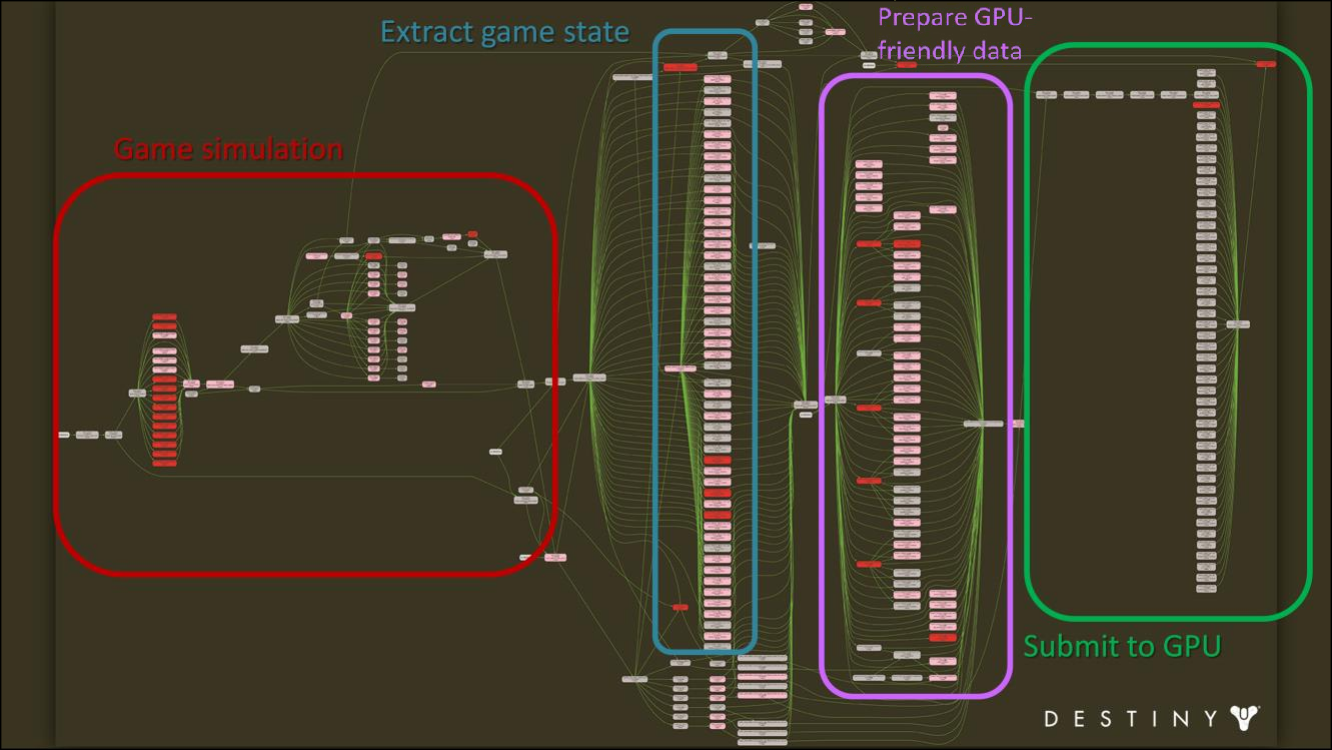
\includegraphics[width=\textwidth]{Destiny.png}
	 \caption{Darstellung eines Job Graphen für das Spiel Destiny. Die farbigen Umrahmungen zeigen die verschieden Stufen, in die der Graph durch Synchronisationspunkte unterteilt ist. Die Abbildung ist eine Aggregation von vier Abbildungen aus \cite[S.~39~ff.]{Tatarchuk2014}.}\label{fig:destiny-jobgraph}
\end{figure}

Im folgenden Kapitel wird nun der Zustand der Blocklib analysiert, um die bereits vorhandene Nutzung von Multithreading zu verstehen und eine Grundlage für das Design der neuen nebenläufigen Architektur und die Anforderungen an diese zu bilden.
\todo{evtl noch schönerer Übergang?}